\subparagraph{UIAPV2 - Introducción a la aplicación} ~\\

\IUDescripcion
[.3] % Width
{adrian/vendedor/prototipoFinal/UIApp/0} % Imagen sin la ruta 'imagen/'
{UIAPVF2} % Identificador
{Introducción a la aplicación.}  % Etiqueta/nombre de la imagen
{Indicar al usuario las funcionalidades que tiene la aplicación y darle a conocer los limites de lo que puede hacer con ella.} %Objetivo
{La figura \ref{UIAPVF2} presenta la pantalla que aparece únicamente la primera vez que se inicia la aplicación, contiene 5 diapositivas en total, las siguientes se muestran en las figuras \ref{UIAPVF2-1} a \ref{UIAPVF2-4} .} %Intro/Breve descripción de la pantalla
{Ninguna.} %Salidas
{Ninguna.} %Entradas


\FloatBarrier
\begin{figure}[htbp!]
		\centering
			
\includegraphics[width=.3 \textwidth]{imagenes/adrian/vendedor/prototipoFinal/UIApp/0_2}
		\caption{Introducción a la aplicación - Ver clientes cercanos}
		\label{UIAPVF2-1}
\end{figure}
\FloatBarrier

\FloatBarrier
\begin{figure}[htbp!]
		\centering
			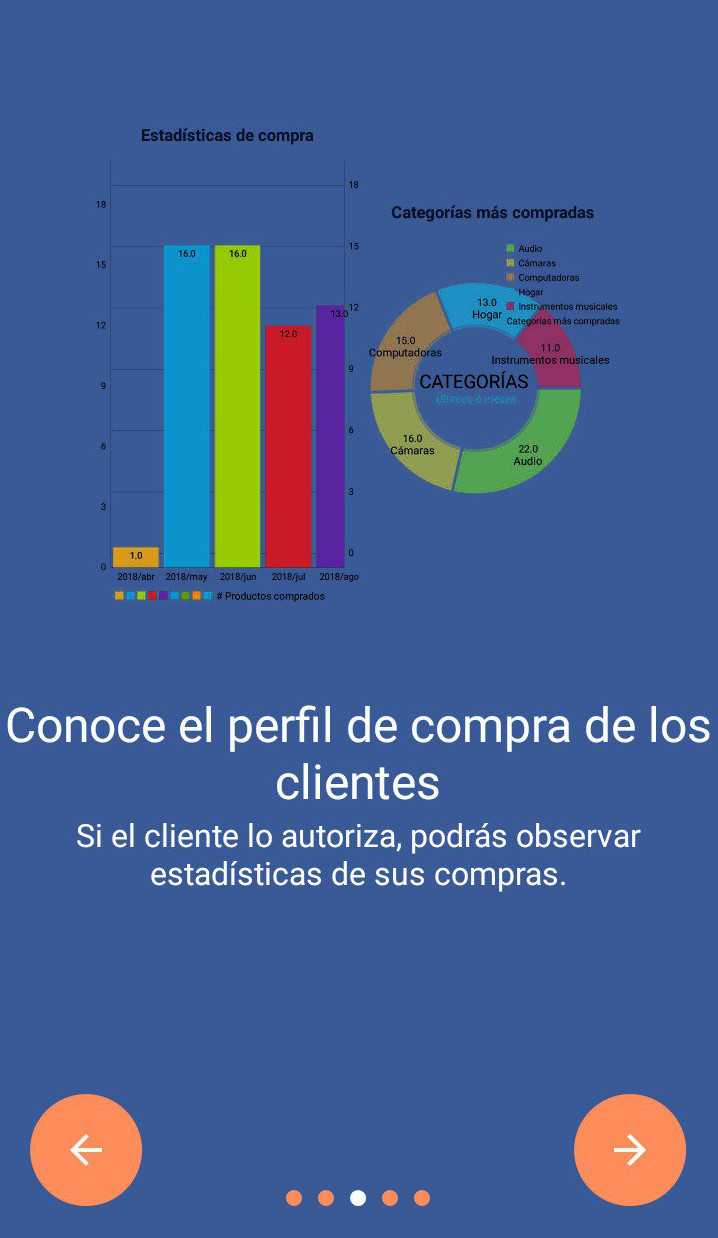
\includegraphics[width=.3 \textwidth]{imagenes/adrian/vendedor/prototipoFinal/UIApp/0_3}
		\caption{Introducción a la aplicación - Perfil de compra de los clientes}
		\label{UIAPVF2-2}
\end{figure}
\FloatBarrier

\FloatBarrier
\begin{figure}[htbp!]
		\centering
			
\includegraphics[width=.3 \textwidth]{imagenes/adrian/vendedor/prototipoFinal/UIApp/0_4}
		\caption{Introducción a la aplicación - Más sobre el cliente}
		\label{UIAPVF2-3}
\end{figure}
\FloatBarrier

\FloatBarrier
\begin{figure}[htbp!]
		\centering
			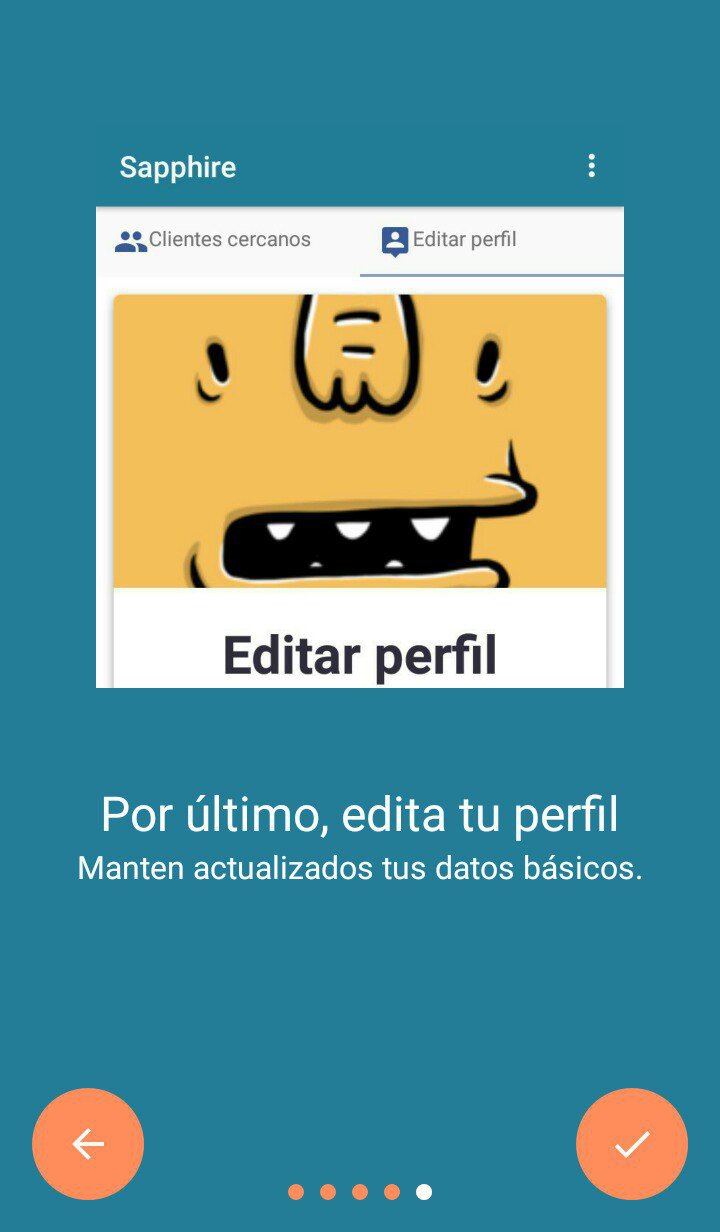
\includegraphics[width=.3 \textwidth]{imagenes/adrian/vendedor/prototipoFinal/UIApp/0_5}
		\caption{Introducción a la aplicación - Editar perfil}
		\label{UIAPVF2-4}
\end{figure}
\FloatBarrier

% Comandos y Mensajes son opcionales